\documentclass[11pt,a4paper]{article}

\usepackage[margin=2.5cm]{geometry}
\usepackage[T1]{fontenc}
\usepackage{lmodern}
\usepackage{graphicx}
\usepackage{booktabs}
\usepackage{float}
\usepackage{caption}
\usepackage{enumitem}
\usepackage{xcolor}
\usepackage{tikz}
\usetikzlibrary{positioning,arrows.meta}
\usepackage[colorlinks=true,linkcolor=black,citecolor=black,urlcolor=blue!50!black]{hyperref}

\graphicspath{{figures/}}
\setlist{itemsep=2pt,topsep=4pt}

\title{\vspace{-3em}
\includegraphics[height=1.5cm]{au_logo.png}\\[0.2em]
{\small School of Engineering and Applied Science, Ahmedabad University}\\[1.2em]
\textbf{SentryCare: AI-Powered Camera Monitoring for\\Resident Safety in Aged Care}\\[0.4em]
\large Final Project Report}
\author{}
\date{}

\begin{document}

\maketitle
\vspace{-3.5em}
\begin{center}
\textbf{Project Track:} Application Based\\[1em]
\begin{tabular}{cc}
\textbf{Kaushalendra Pratap Singh} & \textbf{Dhruv Jain} \\
AU2644013 & AU2644029 \\[0.8em]
\textbf{Nandish Bhatt} & \textbf{Dev Upadhyay} \\
AU2644012 & AU2644003 \\
\end{tabular}\\[1em]
\small Code: \url{https://github.com/sploitengineer/SentryCare}
\end{center}

\begin{abstract}
Falls are one of the most serious risks for older adults in care homes, yet most existing CCTV cameras are used
only to record, not to watch. We built \emph{SentryCare}, a system that turns ordinary cameras (a laptop webcam, a
mobile phone, or an IP/CCTV camera) into an active safety monitor that runs on a normal laptop CPU. SentryCare
recognises enrolled residents and staff, labels anyone else as \emph{Unknown}, tracks every person in view with a
pose model, decides for each person whether a fall has happened, and immediately alerts caretakers on every
connected screen and, optionally, on their phones. Compared with our milestone prototype (one person, MediaPipe pose),
the final system tracks multiple people and adds three rules that make fall detection more robust. On 26 test videos
from the public UR Fall Detection dataset it detected 9 of 13 falls with no false alarms on 13 normal-activity videos,
against 7 of 13 falls and one false alarm for the earlier version. Face matching correctly identified 16 of 16
held-out photos and rejected 16 of 16 as unknown when the person was not enrolled. All data stays on the local
machine.
\end{abstract}

\section{Introduction and Problem Statement}

Care homes already have CCTV cameras, but footage is usually checked only after an incident. If a resident falls
when no staff member is nearby, help can be delayed, and a long time on the floor makes the outcome worse. Wearable
fall sensors exist, but residents (especially those with memory problems) often forget to wear them or take them off.

Our goal was to build a camera-based assistant that \emph{watches} instead of only recording:
it should run on hardware a care home already has, recognise who is in the room, detect falls quickly and reliably,
and alert caretakers immediately, while keeping residents' personal data private.

\section{Objectives}

The objectives set in our milestone proposal, and what we delivered:

\begin{itemize}[leftmargin=*]
  \item \textbf{Use existing cameras.} Delivered: laptop webcams, phones (through the browser, no app) and IP/RTSP cameras,
        all on one dashboard.
  \item \textbf{Identify residents and strangers.} Delivered: guided multi-angle enrolment and face recognition that
        names enrolled people and labels everyone else \emph{Unknown}.
  \item \textbf{Real-time fall detection with few false alarms.} Delivered and extended: multiple people are tracked at
        once, each with their own fall check, plus rules that cut false alarms.
  \item \textbf{Automated alerts.} Delivered: instant alarms on every open dashboard with a snapshot, shared
        acknowledgement, an event log, and optional phone push notifications.
  \item \textbf{Low cost.} Delivered: everything runs on a laptop CPU. The GPU and cloud tier from the proposal was
        \emph{not} needed for this prototype and is left as future work.
\end{itemize}

\section{Related Work}

\textbf{Wearable sensors} detect falls well but depend on residents wearing them. \textbf{Smart cameras} with built-in
analytics require replacing existing cameras. \textbf{Cloud video analytics} running deep models on every frame are
expensive at scale. Classic computer-vision fall detectors that use only the shape of a person's bounding box raise
false alarms when someone simply bends or lies down~\cite{kwolek2014}. Modern pose estimators such as
MediaPipe~\cite{lugaresi2019} and YOLO-pose~\cite{yolo11} give body keypoints in real time, and multi-object trackers
such as ByteTrack~\cite{bytetrack} keep identities across frames. For faces, light-weight models like
YuNet~\cite{yunet} (detection) and SFace~\cite{sface} (recognition) run fast on a CPU. SentryCare combines these
building blocks with temporal rules designed for falls.

\section{System Overview}

Figure~\ref{fig:arch} shows the system. A Flask web server receives frames from each camera. For every camera only
the \emph{newest} frame is kept, so when analysis is slower than the camera, old frames are dropped instead of piling
up; the video stays smooth and alerts are never delayed by a backlog. Each frame goes through a face pipeline and a
body pipeline. Their results are combined per person, stored in a local SQLite database, and confirmed falls are sent to
an alert hub that notifies every open dashboard.

\begin{figure}[H]
\centering
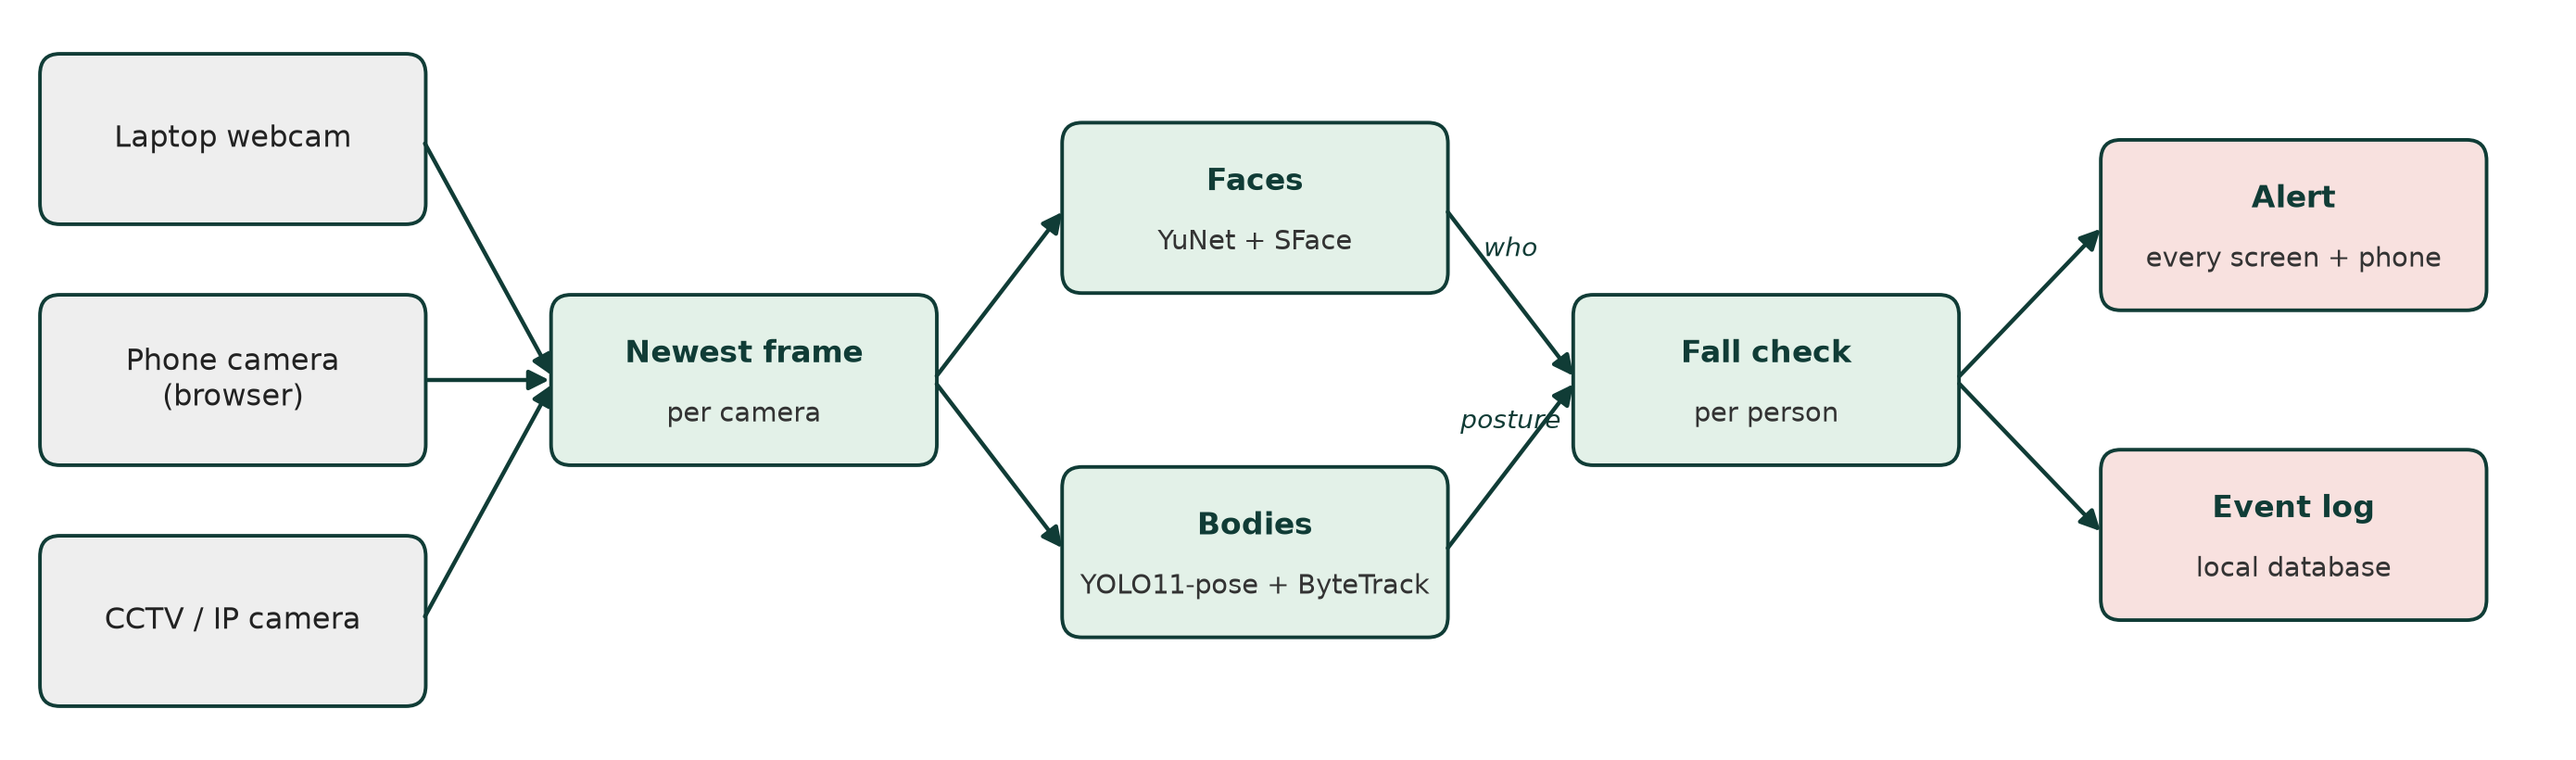
\includegraphics[width=\linewidth]{architecture.png}
\caption{SentryCare architecture. All components run locally on one laptop CPU.}
\label{fig:arch}
\end{figure}

\section{Methodology}

\subsection{Face recognition}

\begin{enumerate}[leftmargin=*]
  \item \textbf{Detect:} YuNet~\cite{yunet} finds each face and five landmarks (eyes, nose, mouth corners).
  \item \textbf{Align:} the face is rotated and cropped the same way every time, using the landmarks.
  \item \textbf{Describe:} SFace~\cite{sface} converts the aligned face into a list of 128 numbers (an
        \emph{embedding}). Photos of the same person produce similar embeddings.
  \item \textbf{Match:} the new embedding is compared with each enrolled person's photos using cosine similarity
        (1 = identical). A name is given only if the best score is at least 0.45, beats the next person by at least
        0.06, and is confirmed on two consecutive checks. Otherwise the face is \emph{Unknown}.
\end{enumerate}

\noindent Enrolment uses guided captures from five angles (or uploads). Every photo is checked automatically: exactly
one face, large enough, sharp, and well lit. At least three accepted photos are needed. We use pretrained models;
``building a profile'' stores embeddings and does not retrain any network.

\subsection{Multi-person fall detection}

For each frame, YOLO11-pose~\cite{yolo11} returns a box and 17 body keypoints for every person, and
ByteTrack~\cite{bytetrack} gives each person a stable ID. Each person then has their own fall check:

\begin{itemize}[leftmargin=*]
  \item \textbf{Posture signals:} how horizontal the torso is, how low the body is in the frame, whether the head is
        below the hips, and how fast the body is moving down.
  \item \textbf{State machine:} \emph{Normal} $\rightarrow$ \emph{Check posture} $\rightarrow$ \emph{Confirming fall}
        $\rightarrow$ \emph{Fall}. A fall must be supported for 1.2\,s before it is confirmed.
  \item \textbf{Stayed-down check:} after confirmation, the person must stay low and roughly still for 2\,s more.
        Getting up cancels the alert.
\end{itemize}

\noindent While testing we found that a person on the floor is often detected poorly: keypoints disappear, or the
tracker loses the person and gives them a new ID. Two rules address this:

\begin{itemize}[leftmargin=*]
  \item \textbf{Box continuation:} if keypoints are lost but the person's box is lying flat \emph{right after} a drop was
        seen, the fall check continues. A missing body alone never counts as a fall.
  \item \textbf{Track hand-off:} if a new person ID appears close to where someone was just lost mid-fall, it takes over
        that person's fall history.
\end{itemize}

\noindent Finally, someone who lies down \emph{without} a drop being seen (for example on a sofa) is shown as
\emph{Lying} and does not trigger an alarm. The earlier single-person MediaPipe~\cite{lugaresi2019} pipeline remains
available as an automatic fallback.

\subsection{Cameras, alerts and privacy}

A phone becomes a camera by opening a link in its browser. Because phones only allow camera access on secure pages,
the system can start an HTTPS link on the local Wi-Fi, protected by a one-time PIN and shown as a QR code. When a fall is
confirmed, every open dashboard shows a full-screen alarm with a snapshot and plays a siren until a caretaker presses
\emph{Acknowledge}, which clears it on all screens. Optional phone push notifications send text only, never images.
Face photos, embeddings and events are stored locally and are blocked from the code repository by automated tests.

\section{Experimental Setup}

\textbf{Fall dataset.} UR Fall Detection Dataset (URFD)~\cite{kwolek2014}, camera 0: 15 fall videos and 15
activities-of-daily-living (ADL) videos such as walking, sitting, crouching and lying on a bed. The dataset gives
frame-level labels of when each fall starts. Clips 01--02 of each type were used during development; clips 03--15
(13 falls, 13 ADLs) form the \textbf{test set}.

\textbf{Protocol.} Videos are processed at 5 frames per second, the same rate as the live system, on a laptop CPU.
URFD videos stop 1--2\,s after the fall, which is too short for a confirmation window plus a stayed-down check. We
therefore report a \textbf{raw} view (video as recorded) and a \textbf{held} view, in which the last frame is repeated
for 4\,s as if the person stays where they are. The held view is applied to both fall and ADL videos, so it does not
favour detection.

\textbf{Metrics.} For each video we check whether an alert was raised. \emph{Recall} is the share of falls detected,
\emph{false alarms} are alerts on ADL videos, and \emph{alert delay} is the time from the labelled start of the fall
to the alert. For faces we use leave-one-out identification, unknown-person rejection, and the true and false accept
rates of photo pairs at different thresholds.

\textbf{Reproducibility.} All experiments are in two Jupyter notebooks in the repository
(\texttt{notebooks/}), and the logged metrics are saved in \texttt{results/}.

\section{Results}

\subsection{Face recognition}

The local test set has 5 enrolled profiles and 16 photos. Photos of the same person have a mean similarity of 0.62,
while photos of different people have a mean of 0.14 (Figure~\ref{fig:face}). The highest score between two different
people was 0.38 and the lowest between two photos of the same person was 0.49, so the 0.45 threshold separates them.

\begin{table}[H]
\centering
\begin{tabular}{lc}
\toprule
Check & Result \\
\midrule
Leave-one-out identification (each photo vs.\ the remaining photos) & 16 / 16 correct \\
Unknown rejection (person removed from the database) & 16 / 16 rejected \\
Same-person pairs accepted at threshold 0.45 (TAR) & 100\% (18 pairs) \\
Different-person pairs accepted at threshold 0.45 (FAR) & 0\% (102 pairs) \\
\bottomrule
\end{tabular}
\caption{Face recognition results on locally enrolled profiles.}
\end{table}

\begin{figure}[H]
\centering
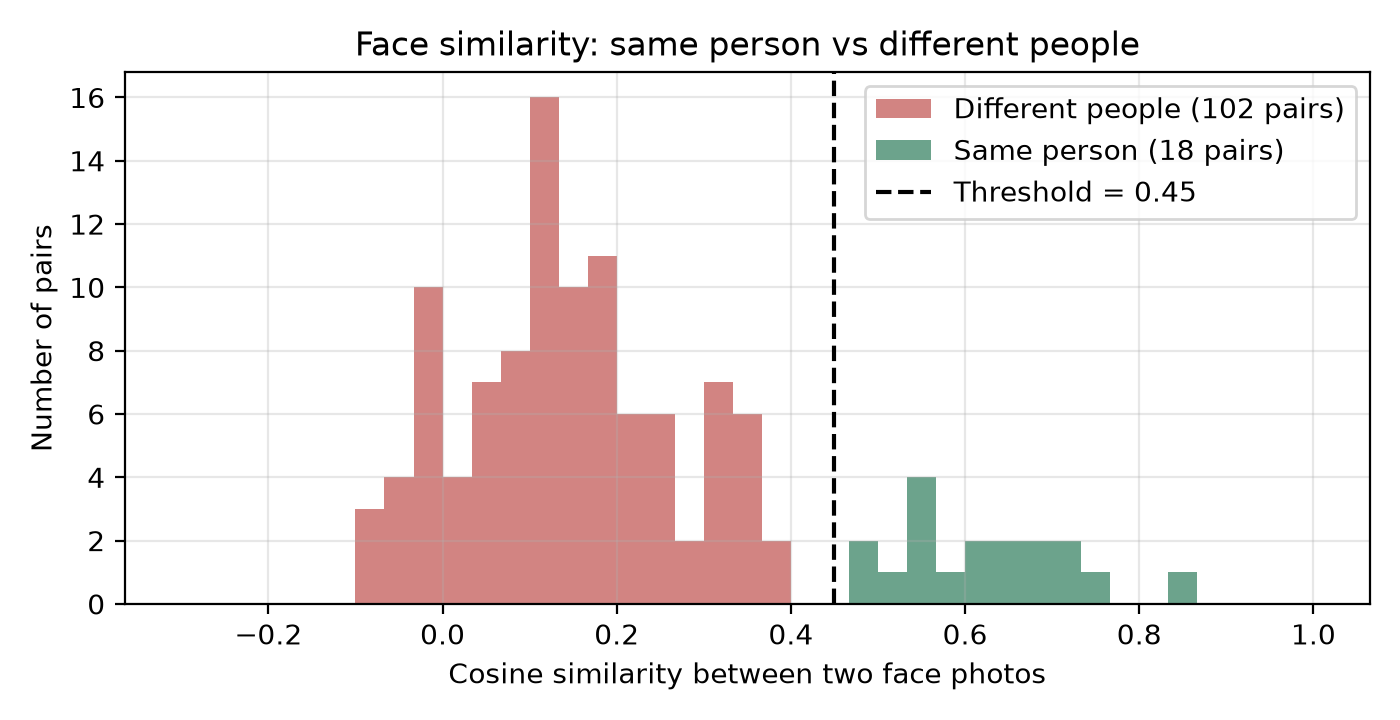
\includegraphics[width=0.49\linewidth]{face_similarity.png}\hfill
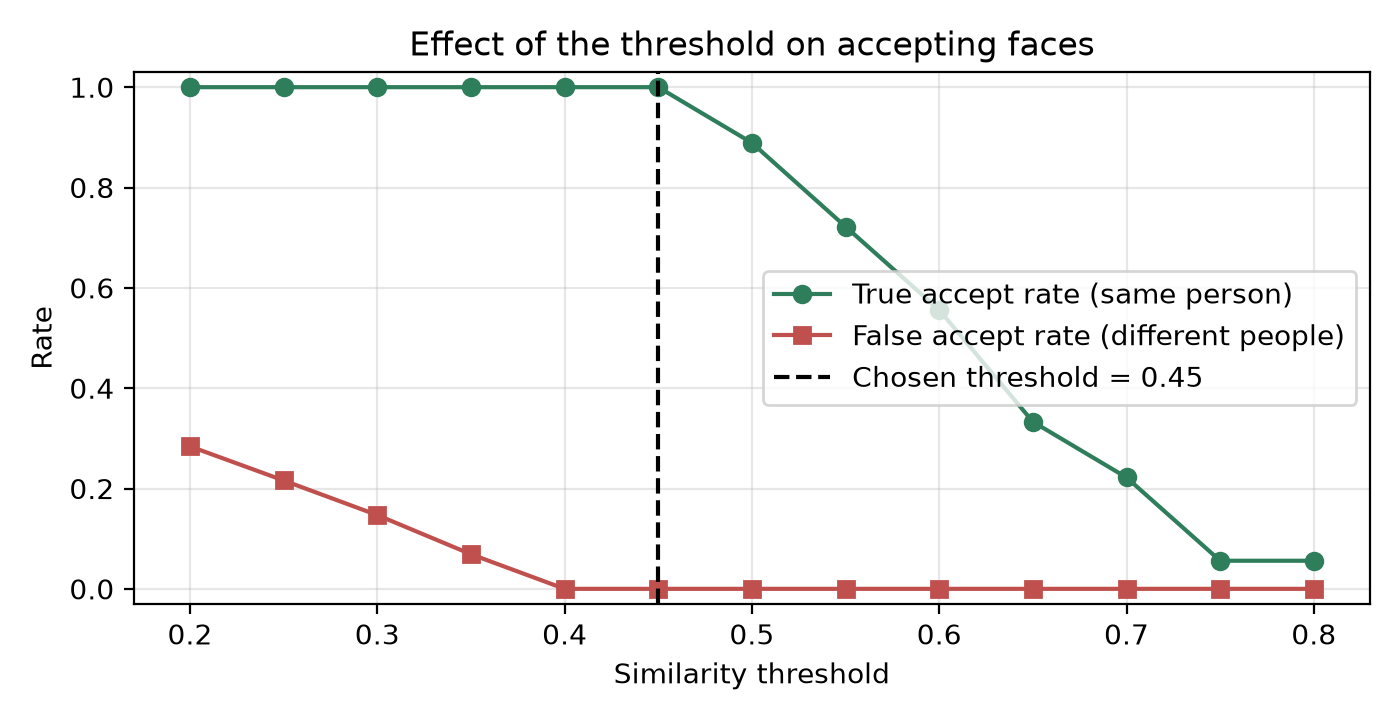
\includegraphics[width=0.49\linewidth]{face_threshold_sweep.png}
\caption{Left: similarity of same-person and different-person photo pairs. Right: effect of the threshold on
accepting faces; 0.45 accepts every same-person pair and no different-person pair.}
\label{fig:face}
\end{figure}

\subsection{Fall detection}

Table~\ref{tab:fall} compares the earlier and the final pipeline. In the held view on the test set, the final system
detects 9 of 13 falls with no false alarms, compared with 7 of 13 and one false alarm before
(Figure~\ref{fig:conf}). In the raw view the final system raises no alerts, because the stayed-down check needs the
person on the floor for about 3\,s after the fall and the recordings end sooner.

\begin{table}[H]
\centering
\begin{tabular}{llcccc}
\toprule
Pipeline & View & Falls detected & False alarms & Precision & F1 \\
\midrule
Earlier: MediaPipe, 1 person & raw  & 3 / 13 & 0 / 13 & 1.00 & 0.38 \\
Earlier: MediaPipe, 1 person & held & 7 / 13 & 1 / 13 & 0.88 & 0.67 \\
Final: YOLO11-pose, multi-person & raw  & 0 / 13 & 0 / 13 & -- & 0.00 \\
\textbf{Final: YOLO11-pose, multi-person} & \textbf{held} & \textbf{9 / 13} & \textbf{0 / 13} & \textbf{1.00} & \textbf{0.82} \\
\bottomrule
\end{tabular}
\caption{Fall detection on the URFD test set (13 fall and 13 ADL videos).}
\label{tab:fall}
\end{table}

\begin{figure}[H]
\centering
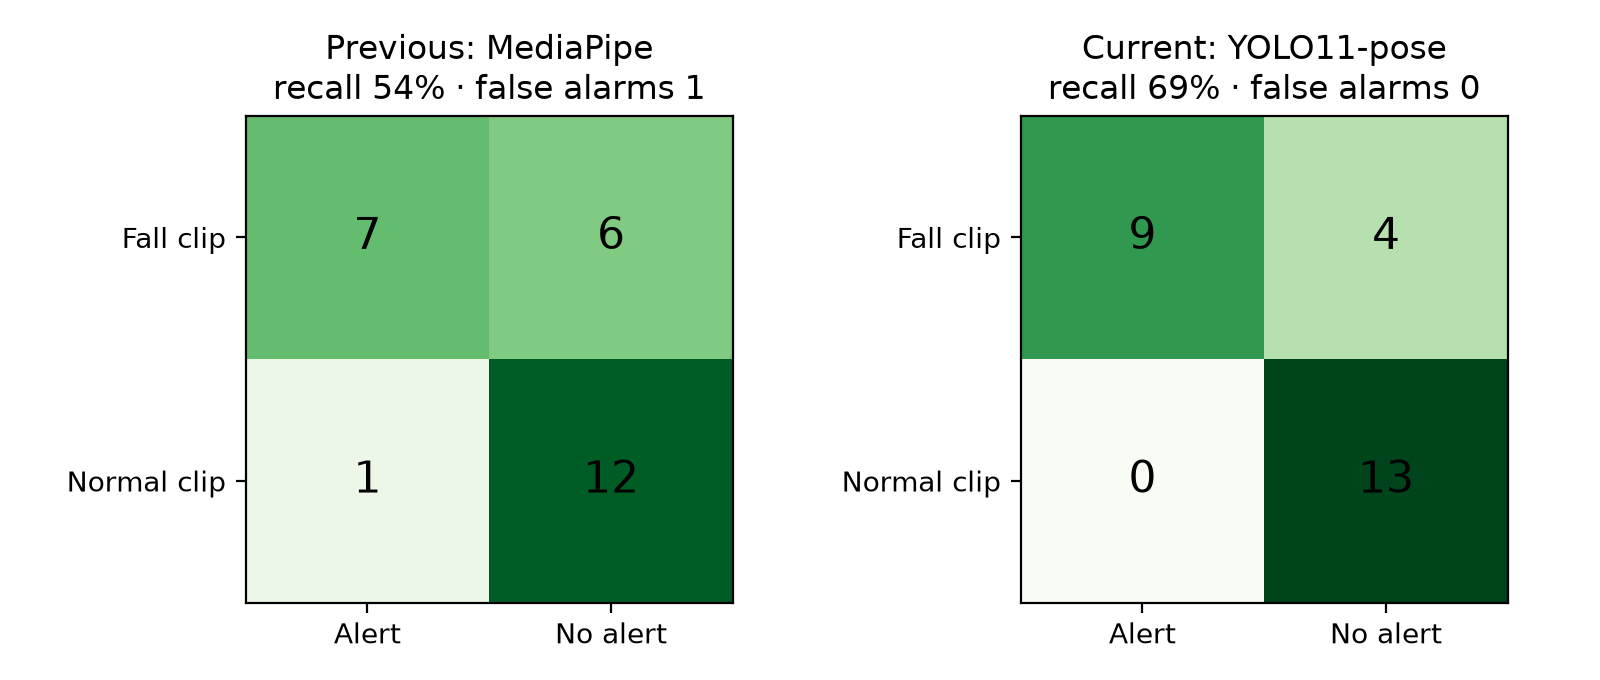
\includegraphics[width=0.62\linewidth]{fall_confusion.png}
\caption{Confusion matrices on the test set (held view).}
\label{fig:conf}
\end{figure}

\textbf{Alert delay.} Measured from the labelled start of the fall, the median delay was 4.4\,s for the final system
(range 3.7--5.7\,s) and 2.6\,s for the earlier one. The extra time is the price of the stayed-down check.
Figure~\ref{fig:timeline} shows one example.

\begin{figure}[H]
\centering
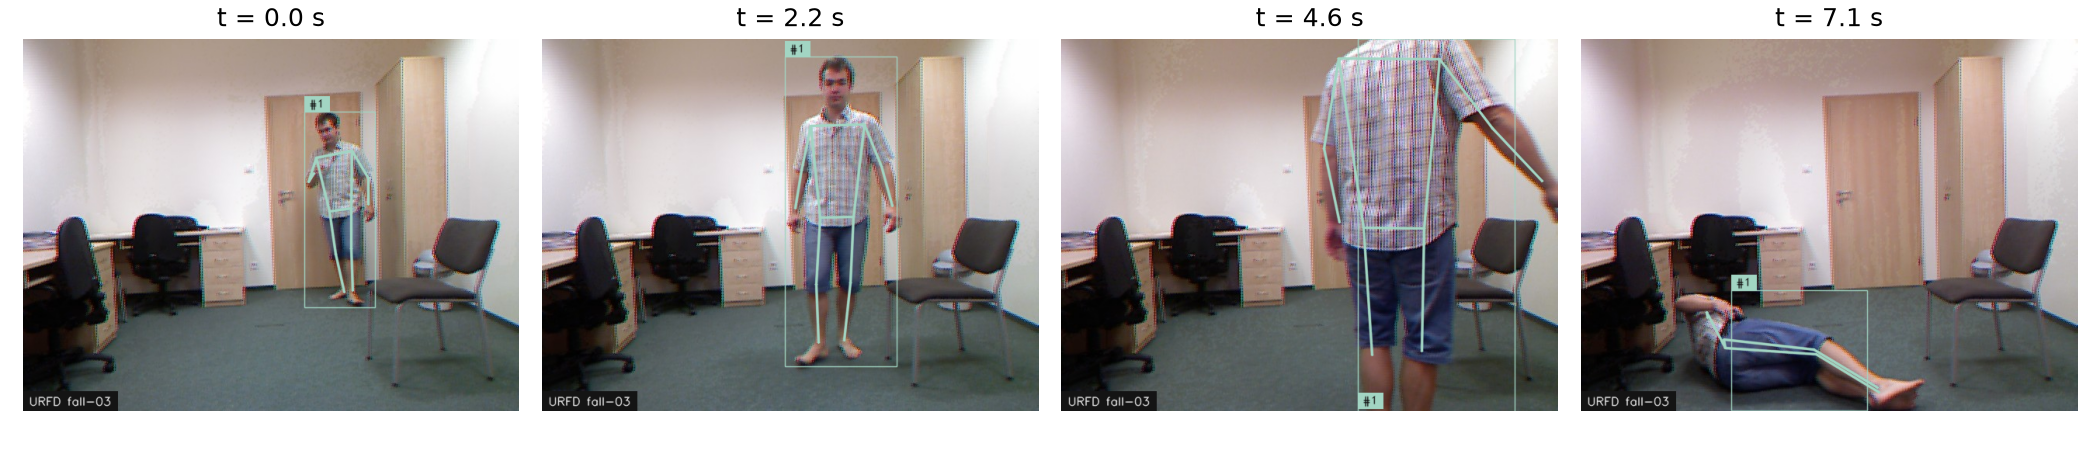
\includegraphics[width=\linewidth]{fall_sequence.png}\\[0.4em]
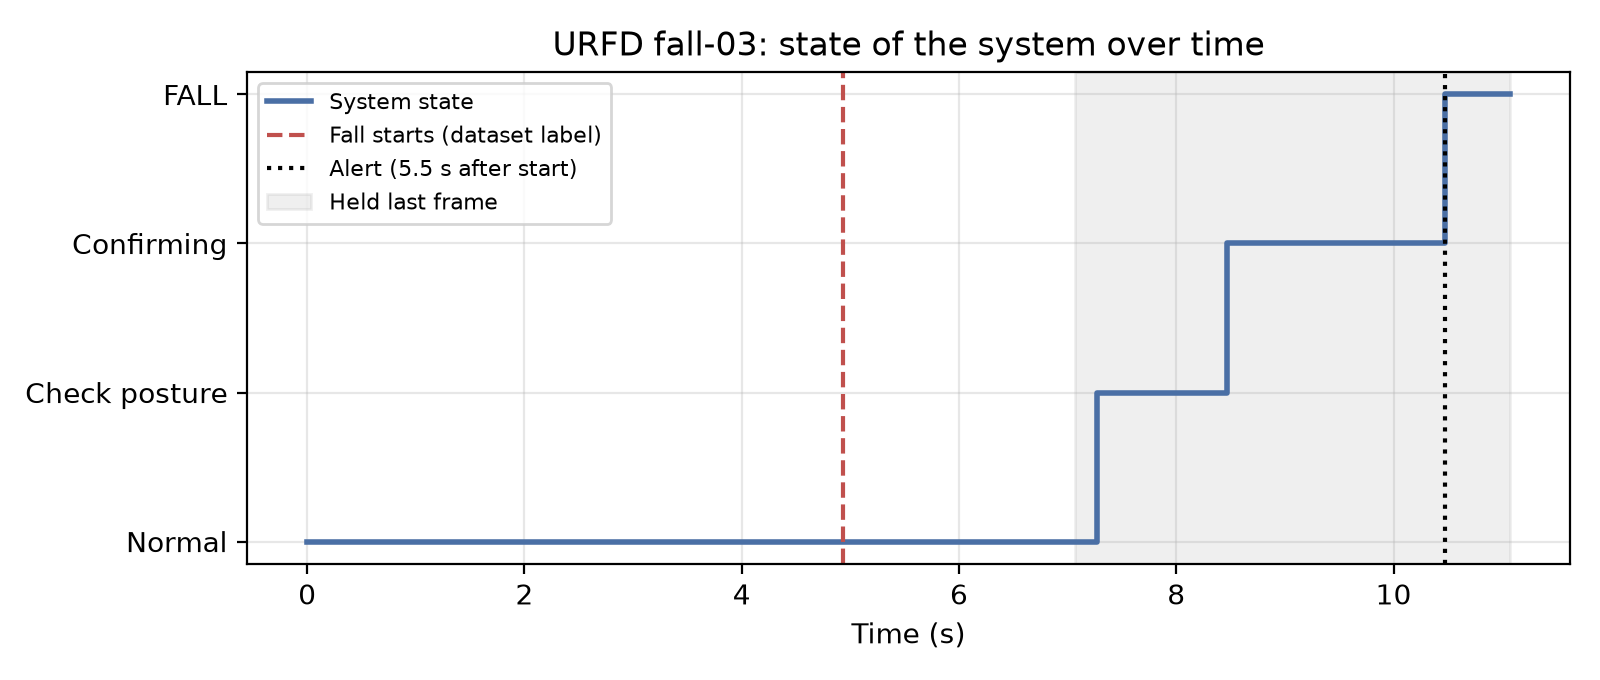
\includegraphics[width=0.72\linewidth]{fall_timeline.png}
\caption{URFD video fall-03. Top: what the system sees (box, skeleton and person ID). Bottom: the system's state over
time; the alert is raised after the person stays down.}
\label{fig:timeline}
\end{figure}

\textbf{Ablation.} Table~\ref{tab:ablation} switches off one rule at a time (all 30 videos, held view). Box
continuation is the most important rule: without it, detected falls drop from 11 to 6. Track hand-off adds two
detected falls. The stayed-down check did not change detection on URFD (Figure~\ref{fig:stay}); it only adds delay.

\begin{table}[H]
\centering
\begin{tabular}{lccc}
\toprule
Variant & Falls detected & False alarms & F1 \\
\midrule
Full system & 11 / 15 & 0 / 15 & 0.85 \\
Without stayed-down check & 11 / 15 & 0 / 15 & 0.85 \\
Without box continuation & 6 / 15 & 0 / 15 & 0.57 \\
Without track hand-off & 9 / 15 & 0 / 15 & 0.75 \\
\bottomrule
\end{tabular}
\caption{Ablation study: contribution of each rule (all 30 videos, held view).}
\label{tab:ablation}
\end{table}

\begin{figure}[H]
\centering
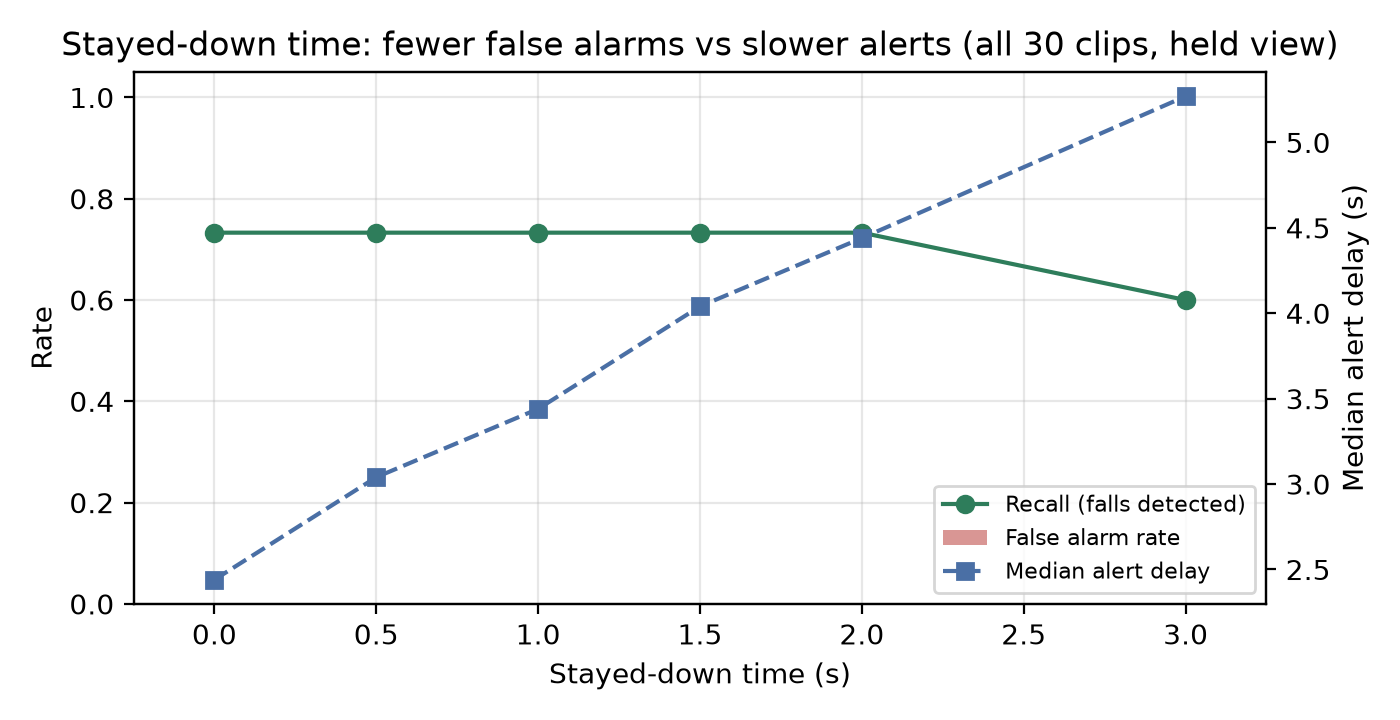
\includegraphics[width=0.66\linewidth]{stay_down_sweep.png}
\caption{Stayed-down time vs.\ detection and delay. On URFD, longer waits only add delay.}
\label{fig:stay}
\end{figure}

\textbf{Speed.} YOLO11-pose with tracking takes about 100\,ms per frame on a laptop CPU (up to about 10 frames per
second) and MediaPipe about 42\,ms. Both are fast enough for the 5 frames per second used by the system.

\section{Discussion and Limitations}

\begin{itemize}[leftmargin=*]
  \item \textbf{Small evaluation.} 26 test videos from one dataset, one camera angle and young actors performing
        staged falls. The results show the direction of improvement, not a validated accuracy.
  \item \textbf{Stayed-down check.} URFD's normal videos contain no ``drop and get straight back up'' moments, so we
        could not measure the false alarms this rule is designed to prevent. A shorter wait (about 1\,s) would reduce
        the delay at little risk.
  \item \textbf{Missed falls.} Four test falls were missed. Studying these cases one by one is part of future work.
  \item \textbf{Live conditions.} The benchmark replays frames under ideal conditions. Live frames are compressed by the
        camera and are sometimes skipped when the computer is busy. When we streamed six fall videos through the
        running dashboard, five raised an alert, so borderline falls can be missed in live use.
  \item \textbf{Unseen falls.} A person who falls outside the camera view and then appears on the floor is shown as
        \emph{Lying} but not alerted, because no drop was observed.
  \item \textbf{Face recognition} was tested only on a few locally enrolled people. It has not been tested on a large
        population, in poor lighting, or against spoofing with printed photos or screens.
  \item \textbf{Deployment.} The prototype runs on a trusted local network. A real deployment would need user accounts,
        a production web server, data-retention rules and staff training.
\end{itemize}

\section{Conclusion and Future Work}

SentryCare shows that ordinary cameras and a laptop CPU are enough to build a useful resident-safety assistant: it
recognises people, tracks several people at once, detects falls with a low false-alarm rate in our tests, and alerts
caretakers instantly on any connected screen, while keeping personal data local. Moving from a single-person
pipeline to multi-person tracking with box continuation and track hand-off increased detected falls from 7 to 9 out of
13 test videos and removed the only false alarm.

Future work: (1) train a model that learns fall patterns from sequences of body keypoints instead of hand-set rules,
using larger datasets such as Le2i; (2) add a ``lying too long'' alert for falls that happen out of view; (3) test face
recognition on more people and add liveness (anti-spoofing) checks; and (4) build the event-driven GPU confirmation
tier and a secure multi-user deployment proposed in the milestone.

\begin{thebibliography}{9}
\bibitem{kwolek2014} B.~Kwolek and M.~Kepski, ``Human fall detection on embedded platform using depth maps and
wireless accelerometer,'' \emph{Computer Methods and Programs in Biomedicine}, vol.~117, no.~3, pp.~489--501, 2014.
\bibitem{lugaresi2019} C.~Lugaresi et al., ``MediaPipe: A framework for building perception pipelines,''
\emph{arXiv:1906.08172}, 2019.
\bibitem{yolo11} G.~Jocher and J.~Qiu, ``Ultralytics YOLO11,'' 2024. [Online]. Available:
\url{https://github.com/ultralytics/ultralytics}
\bibitem{bytetrack} Y.~Zhang et al., ``ByteTrack: Multi-object tracking by associating every detection box,''
in \emph{Proc. European Conference on Computer Vision (ECCV)}, 2022.
\bibitem{yunet} W.~Wu, H.~Peng and S.~Yu, ``YuNet: A tiny millisecond-level face detector,''
\emph{Machine Intelligence Research}, vol.~20, pp.~656--665, 2023.
\bibitem{sface} Y.~Zhong et al., ``SFace: Sigmoid-constrained hypersphere loss for robust face recognition,''
\emph{IEEE Transactions on Image Processing}, vol.~30, pp.~2587--2598, 2021.
\end{thebibliography}

\end{document}
